\documentclass[border=2mm,tikz]{standalone}
\usepackage{tikz}
\usetikzlibrary{calc}

\begin{document}

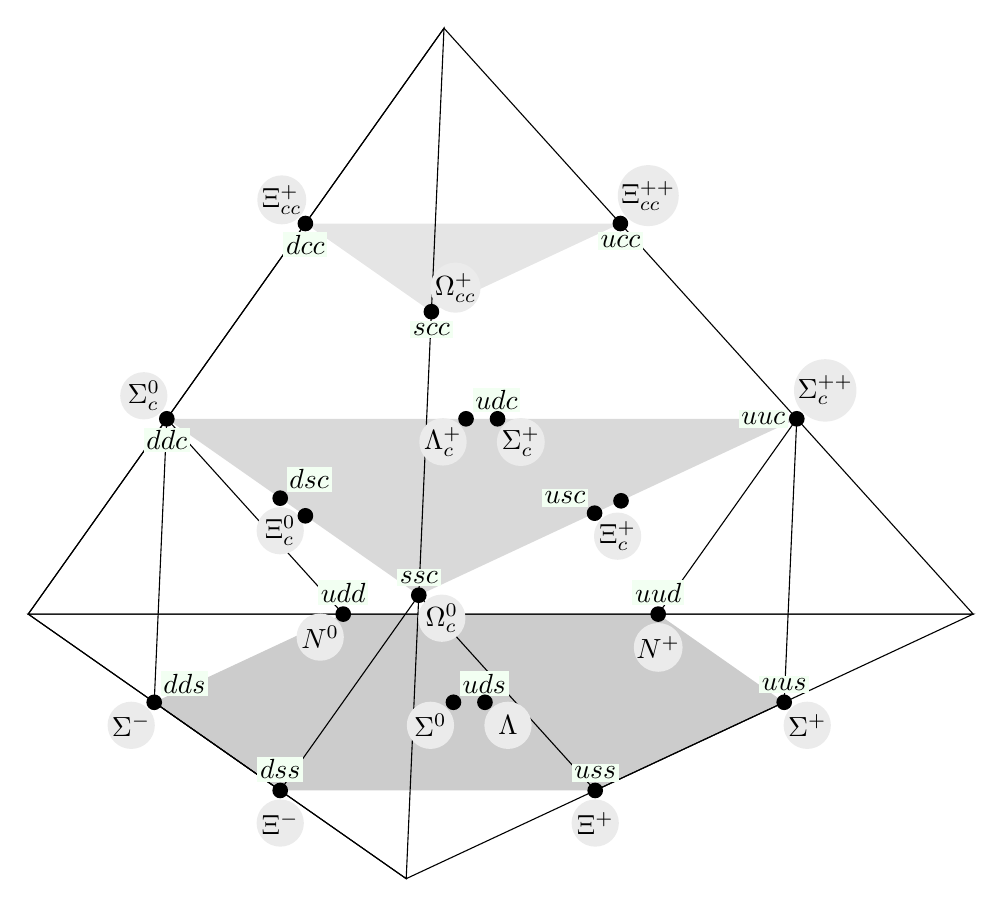
\begin{tikzpicture}[
                x={(5cm,0cm)},y={(2cm,-1.4cm)},z={(2.2cm,3.1cm)},scale=0.8,
                Dot/.style={circle,fill=black,inner sep=2pt, pin distance=0pt},
                lab/.style={circle,fill=black!8,inner sep=0pt,minimum size=6mm},
                qua/.style={fill=green!5,inner sep=1pt}
        ]
%
%
\coordinate (ddd) at (0,0,0);
\coordinate (udd) at (1,0,0);
\coordinate (uud) at (2,0,0);
\coordinate (uuu) at (3,0,0);
%
\coordinate (dds) at (0,1,0);
\coordinate (uds) at (1,1,0);
\coordinate (uus) at (2,1,0);
%
\coordinate (dss) at (0,2,0);
\coordinate (uss) at (1,2,0);
%
\coordinate (sss) at (0,3,0);
%
\fill[black!20] (udd) -- (uud) -- (uus) -- (uss) -- (dss) -- (dds) -- cycle;
%
\coordinate (ddc) at (0,0,1);
\coordinate (udc) at (1,0,1);
\coordinate (uuc) at (2,0,1);
%
%
\coordinate (dsc) at (0,1,1);
\coordinate (usc) at (1,1,1);
%
\coordinate (ssc) at (0,2,1);
%
\fill[black!15] (ddc) -- (uuc) -- (ssc) -- cycle;
%
\coordinate (dcc) at (0,0,2);
\coordinate (ucc) at (1,0,2);
\coordinate (scc) at (0,1,2);
%
\fill[black!10] (dcc) -- (ucc) --  (scc) -- cycle;
%
\coordinate (ccc) at (0,0,3);
%
\draw (ddd) -- (uuu) -- (ccc) -- cycle;
\draw (ddd) -- (sss) -- (uuu) -- cycle;
\draw (ddd) -- (sss) -- (ccc) -- cycle;
\draw (udd) -- (ddc) -- (dds) -- (dss) -- (ssc) -- (uss) -- (uus) -- (uuc) -- (uud);





        \node [Dot, label={[lab]below left:$N^0$},label={[qua]above:$udd$}]       (neutron) at (udd) {};
        \node [Dot, label={[lab]below:$N^+$},label={[qua]above:$uud$}]            (proton)  at (uud) {};
        \node [Dot, label={[lab]below left:$\Sigma^-$},label={[qua]above right:$dds$}]  (sigMin)  at (dds) {};
        \node [Dot, label={[lab]below left:$\Sigma^0$},label={[qua]above right:$uds$}]  (sigZer)  at ($ (uds)-(0.05,0,0) $) {};
        \node [Dot, label={[lab]below right:$\Lambda$}]  (lamZer)  at ($ (uds)+(0.05,0,0) $) {};
        \node [Dot, label={[lab]below right:$\Sigma^+$},label={[qua]above:$uus$}] (sigPlu)  at (uus) {};
        \node [Dot, label={[lab]below:$\Xi^-$},label={[qua]above:$dss$}]          (xiMin)   at (dss) {};
        \node [Dot, label={[lab]below:$\Xi^+$},label={[qua]above:$uss$}]          (xiPlu)   at (uss) {};
%
        \node [Dot, label={[lab]above left:$\Sigma^0_c$},label={[qua]below:$ddc$}]  (CsigZer) at (ddc) {};
        \node [Dot, label={[lab]below left:$\Lambda^+_c$},label={[qua]above right:$udc$}] (ClamPlu) at ($ (udc)-(0.05,0,0) $) {};
        \node [Dot, label={[lab]below right:$\Sigma^+_c$}] (CsigPlu) at ($ (udc)+(0.05,0,0) $) {};
        \node [Dot, label={[lab]above right:$\Sigma^{++}_c$},label={[qua]left:$uuc$}] (CsigPlu2) at (uuc) {};
        \node [Dot, label={[lab]below:$\Xi^0_c$},label={[qua]above right:$dsc$}]     (CxiZer)  at ($ (dsc)-(0,0.1,0) $) {};
        \node [Dot]                                       (CxiZer_) at ($ (dsc)+(0,0.1,0) $) {};
        \node [Dot, label={[lab]below right:$\Xi^+_c$},label={[qua]above left:$usc$}]    (CxiPlu)  at ($ (usc)-(0.07,-0.07,0) $) {};
        \node [Dot]                                       (CxiPlu_) at ($ (usc)+(0.07,-0.07,0) $) {};
        \node [Dot, label={[lab]below right:$\Omega^0_c$},label={[qua]above:$ssc$}]       (ComeZer) at (ssc) {};
%
        \node [Dot, label={[lab]above left:$\Xi^+_{cc}$},label={[qua]below:$dcc$}]    (CCxiPlu)  at (dcc) {};
        \node [Dot, label={[lab]above right:$\Xi^{++}_{cc}$},label={[qua]below:$ucc$}] (CCxiPlu2) at (ucc) {};
        \node [Dot, label={[lab]above right:$\Omega^{+}_{cc}$},label={[qua]below:$scc$}]  (CComePlu)   at (scc) {};
%
\end{tikzpicture}

\end{document}